\documentclass[aspectratio=169]{beamer}
\usetheme{Madrid}
\usecolortheme{beaver}
\usepackage[utf8]{inputenc}
\usepackage[T1]{fontenc}
\usepackage{tikz}
\usepackage{amssymb}
\usepackage{graphicx}
\setbeamertemplate{navigation symbols}{}
\setbeamercolor{title}{fg=white,bg=blue!55!black}
\setbeamercolor{frametitle}{fg=white,bg=blue!45!black}
\setbeamercolor{block title}{bg=blue!15,fg=black}
\setbeamercolor{block body}{bg=blue!5,fg=black}

\title{M6 — Files \& Data}
\subtitle{Reading/writing CSV, mean/max/min, a chart from real data}
\author{ByteForge --- Grade 8 --- App Builder}
\date{}

\begin{document}

\begin{frame}
    \titlepage
\end{frame}

\begin{frame}{Today's Plan}
    \begin{itemize}
        \item Opening a Real File
        \item Built-in Stats Functions
        \item Binary Search
        \item Linking Two Datasets
        \item Append vs. Write Mode
        \item The Whole Pipeline
        \item[$\bigstar$] BOSS --- M6 Capstone
    \end{itemize}
\end{frame}

\begin{frame}{Opening and reading a real file}
    \Large
    \texttt{open("students.csv")} opens a real file; \texttt{.readlines()} gives every line as a list of strings. \texttt{lines[1:]} skips the header row.
\end{frame}


\begin{frame}{Built-in stats functions on real data}
    \Large
    \texttt{max()}, \texttt{min()}, \texttt{sum()}, \texttt{len()} do the heavy lifting once your data is in a real list — exactly what a spreadsheet's AVERAGE/MAX/MIN/COUNT do.
\end{frame}


\begin{frame}{Binary search — a real, faster search}
    \Large
    Instead of checking one by one, binary search jumps to the MIDDLE of a sorted list — an entire HALF can be thrown away every step. Only works because the data is SORTED.

    \begin{center}
    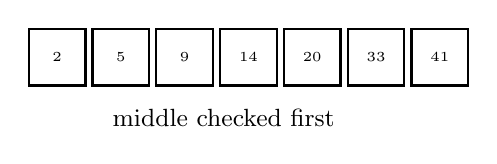
\begin{tikzpicture}[scale=0.9]

        \foreach \x/\v in {0/2,1/5,2/9,3/14,4/20,5/33,6/41} {
          \draw[thick] (\x*0.9,0) rectangle (\x*0.9+0.8,-0.8);
          \node at (\x*0.9+0.4,-0.4) {\tiny \v};
        }
        \node[below] at (2.75,-1) {\small middle checked first};
    \end{tikzpicture}
    \end{center}
\end{frame}


\begin{frame}{Append mode ("a") vs. write mode ("w")}
    \Large
    "w" WIPES a file clean every time; "a" adds to the END, leaving everything already there untouched — exactly how a real log file works.
\end{frame}

\begin{frame}{Real-World Example}
    \Large
    Every school's real student database links a roster file to a results file by a shared student ID — exactly M6's "linking two datasets by a shared key", the same idea behind a real database JOIN.
\end{frame}


\begin{frame}{Let Them Discover}
    \Large
    Open any spreadsheet you have access to. Find its "header row" — the one that isn't data, just column names. Real code has to explicitly skip that row, the same way \texttt{lines[1:]} does here.
\end{frame}

\begin{frame}{Your Turn}
    \Large
    Open the student map, find \textbf{M6 — Files \& Data}, and work through it
    hands-on --- everything you just saw, they now do themselves.
\end{frame}

\end{document}
